\documentclass[12pt,a4paper]{article}

\usepackage{german}      % Deutsche TeX-Eigenheiten
%\usepackage{isolatin1}   % Eingabekodierung mit Umlauten...

\usepackage{makeidx}
\makeindex            % damit eine Indexdatei angelegt wird

\usepackage{graphicx}

\usepackage{amsmath}  % allgemeine Mathe-Erweiterungen
\usepackage{amssymb}  % Symbole und Schriftarten
\usepackage{amsthm}   % erweiterte Theorem-Umgebungen

\usepackage{mathrsfs}  % gibt den Befehl "\mathscr{}" f�r sch�ne

\begin{document}

\section{21. Die Taylorsche Formel}
Funktion = Summe eines Polynoms + Fehlerterm (Restglied) \\
Problem: Funktionen auf Rechner darstellen ( sin,cos,Expo,..)\\
Grundidee:\\
f(x) durch Polynom Pn(x) approximieren (annähern)\\
Polynom :\\
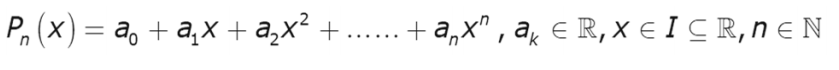
\includegraphics[width=1\textwidth]{Bilder/V1/1.png}
1. Forderung 0 ist im Intervall enthalten\\
Ansatz:\\
Wert von f an der Stelle x (exakt)\\
\= Näherung + Rest\\
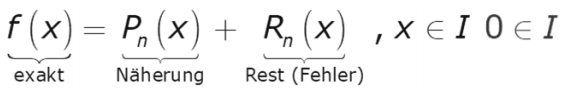
\includegraphics[width=0.5\textwidth]{Bilder/V1/2.png}
\\
Weitere Forderung:\\
an der Stelle 0 soll der Funktionswert und der Wert der k'ten Ableitung von k=0 (0.ableitung)\\
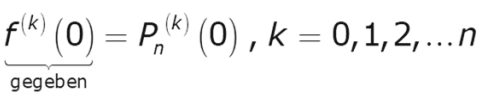
\includegraphics[width=0.4\textwidth]{Bilder/V1/3.png}\\
k'te Ableitung eines Polynoms:\\
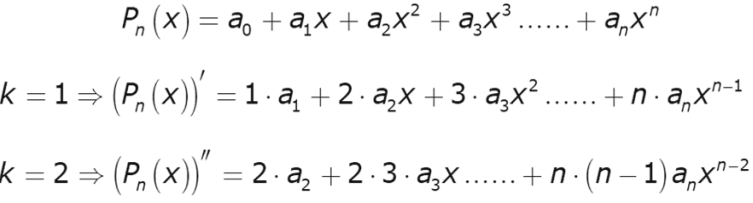
\includegraphics[width=0.5\textwidth]{Bilder/V1/4.png}
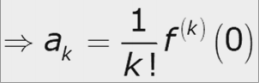
\includegraphics[width=0.3\textwidth]{Bilder/V1/5.png}

\subsubsection{Näherungspolynom}
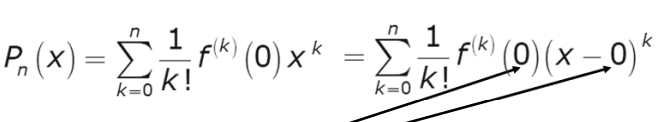
\includegraphics[width=0.5\textwidth]{Bilder/V1/6.png}\\
Stelle 0 geht als Funktionswert ein\\
Wenn x(hoch)k \= (x-0)(hoch)k\\
Problem: 0 nicht im Intervall ?\\
Forderung ist gleich, bzw bezieht sich auf x0\\
= (x-x0)(hoch)k\\
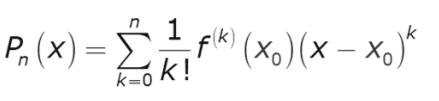
\includegraphics[width=0.4\textwidth]{Bilder/V1/7.png}

\subsection{Satz von Taylor}
Funktion f soll in einem Intervall, n+1 mal stetig differenzierbar sein.\\
d.h. Ableitungen existieren und sind stetig\\
Formel:\\
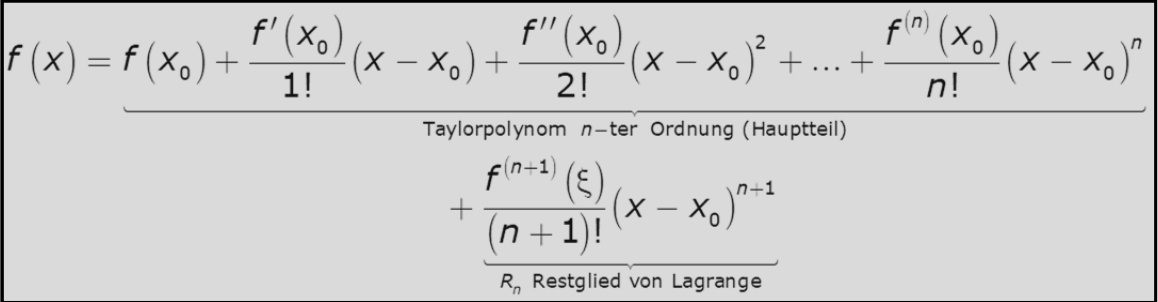
\includegraphics[width=1\textwidth]{Bilder/V1/8.png}\\
Entwicklungspunkt x0 = beliebig, aber fest aus Intervall\\
Zwischenstelle *Symbol* liegt zwischen x und x0, kann also kleiner als x oder auch größer sein.\\
\subsubsection{Fehlerabschätzung}
n+1. Ableitung beschänkt im Intervall I.\\
= Für alle x aus I der Betrag der n+1 Ableitung von f an der Stelle x kleiner 0 einer Konstanten ist\\
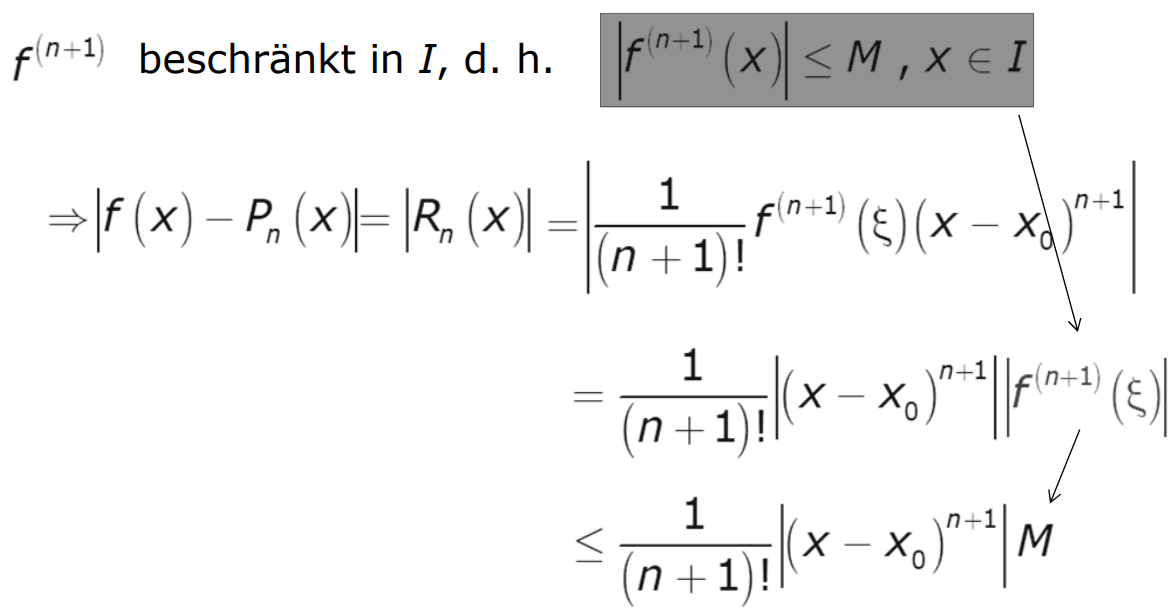
\includegraphics[width=1\textwidth]{Bilder/V1/9.png}\\
Man sieht:\\
1. Je größer das n, dest kleiner wird der Faktor 1 (1/(1-n)!)\\
auf Deutsch: mit Großerem n wird die approximation besser\\
2. Je weiter das x von x0 weg liegt, desto größer wird der Bertrag x-x0, \\
desto mehr Einfluss hat der Term auf die Genauigkeit\\
\subsubsection{Beispiel 1}
Die Berechnung von Wurzeln - Wurzel(42)\\
mit TaylorPolynom 1. Ordnung; Entwicklungspunkt x0 größer 0\\
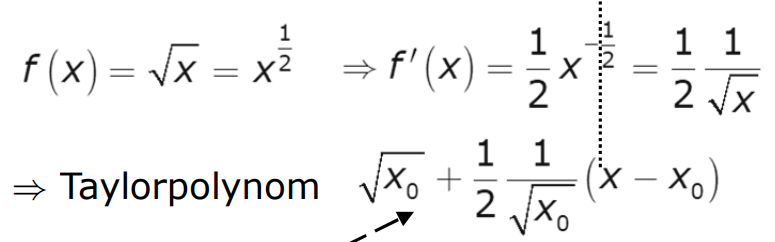
\includegraphics[width=1\textwidth]{Bilder/V1/10.png}\\
setzten x ein (Wurzel(42)) und bestimmen x0 = 36\\
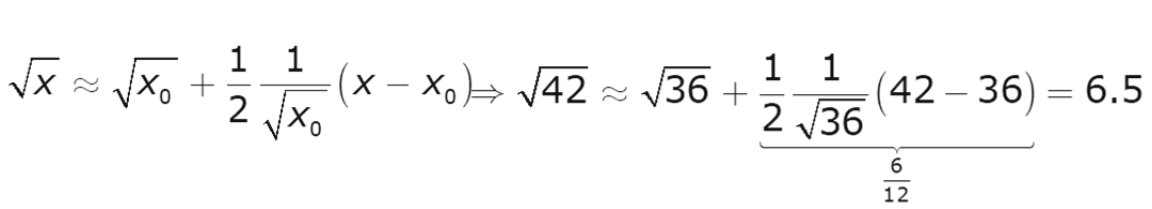
\includegraphics[width=1\textwidth]{Bilder/V1/11.png}\\
Umstellen für Fehlerabschätzung des Restglieds\\
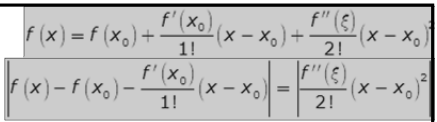
\includegraphics[width=1\textwidth]{Bilder/V1/12.png}\\
Fehlerabschätzung des Restglieds 
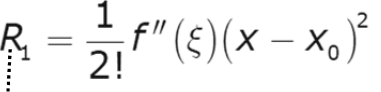
\includegraphics[width=0.5\textwidth]{Bilder/V1/13.png}\\
Brauchen 2. Ableitung\\
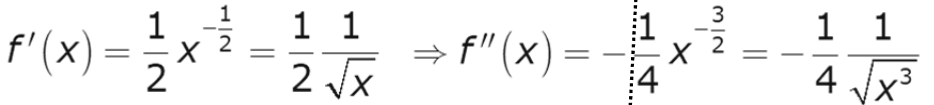
\includegraphics[width=1\textwidth]{Bilder/V1/14.png}\\
\newpage
Dann einsetzten, ergibt:\\
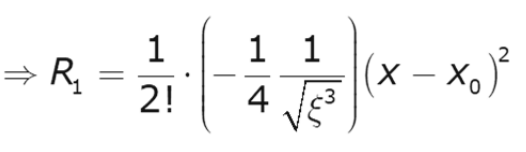
\includegraphics[width=1\textwidth]{Bilder/V1/15.png}\\
Umstellen und einsetzten:\\
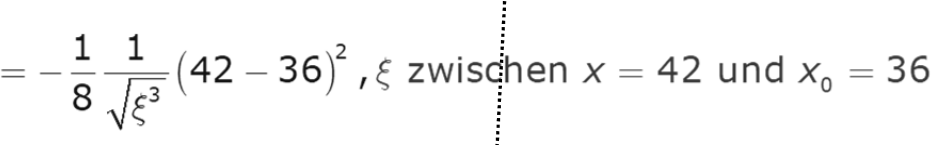
\includegraphics[width=1\textwidth]{Bilder/V1/16.png}\\
Jetzt alles zusammen packen:\\
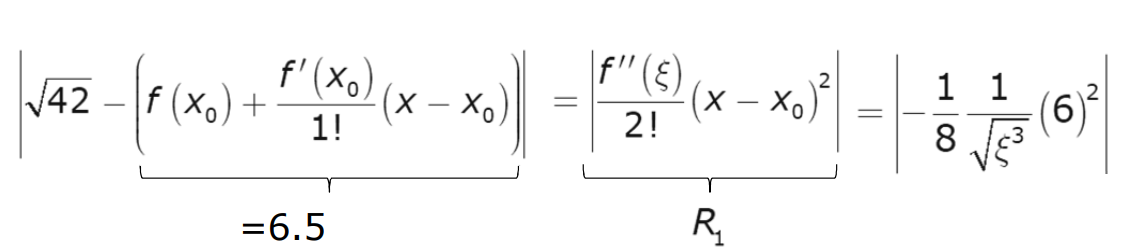
\includegraphics[width=1\textwidth]{Bilder/V1/17.png}\\
Den Abschnitt mit XI[ksi] verkürzen\\
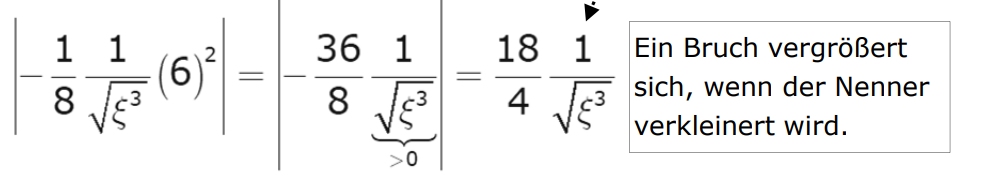
\includegraphics[width=1\textwidth]{Bilder/V1/18.png}\\
Der Schlimmste Fall ist, wenn XI gleich X0, also 36 ist:\\
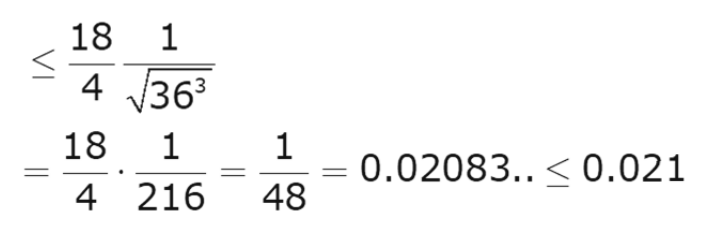
\includegraphics[width=1\textwidth]{Bilder/V1/19.png}\\
Zusammenfassung:\\
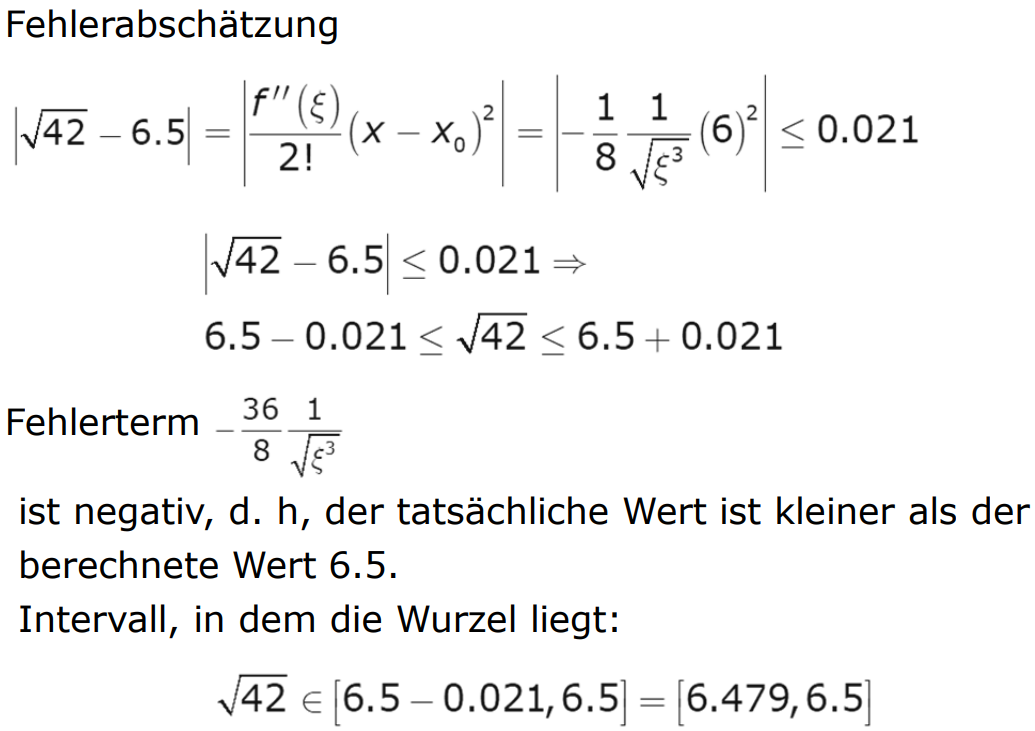
\includegraphics[width=1\textwidth]{Bilder/V1/20.png}\\
\subsubsection{Beispiel 2}
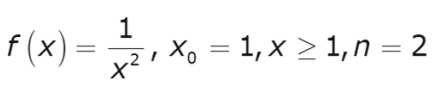
\includegraphics[width=0.5\textwidth]{Bilder/V1/21.png}\\
1. Schritt: Ableitungen + x0 einsetzten\\
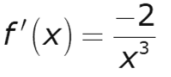
\includegraphics[width=0.3\textwidth]{Bilder/V1/22.png}
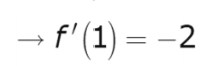
\includegraphics[width=0.3\textwidth]{Bilder/V1/22_1.png}\\
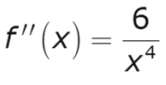
\includegraphics[width=0.3\textwidth]{Bilder/V1/23.png}
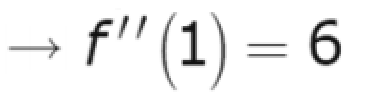
\includegraphics[width=0.3\textwidth]{Bilder/V1/23_1.png}\\
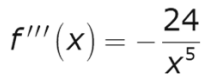
\includegraphics[width=0.35\textwidth]{Bilder/V1/24.png}
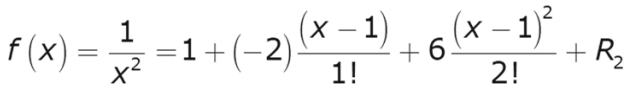
\includegraphics[width=0.9\textwidth]{Bilder/V1/25.png}\\\\
\newpage
Nun kommt die Fehlerabschätzung des Restglieds:\\
Erstmal wieder Kürzen:\\
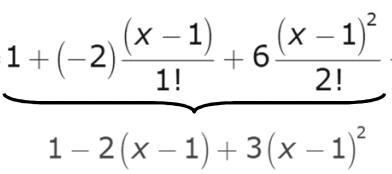
\includegraphics[width=0.5\textwidth]{Bilder/V1/26.png}\\
Mit dem Restglied:\\
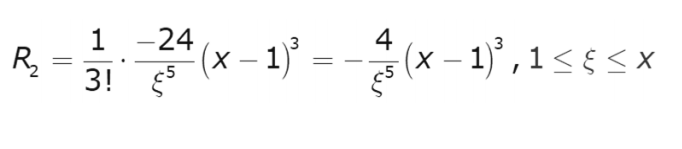
\includegraphics[width=0.8\textwidth]{Bilder/V1/27.png}\\
Und die Abschätzung: eig 1 Einsetzten und schauen, was passiert\\
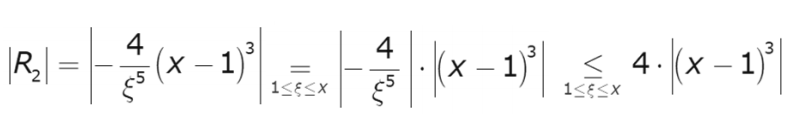
\includegraphics[width=0.8\textwidth]{Bilder/V1/28.png}\\
\newpage
\subsubsection{Beispiel 3}
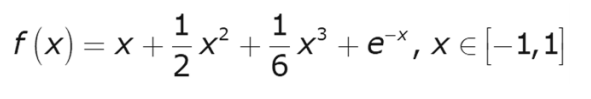
\includegraphics[width=0.5\textwidth]{Bilder/V1/29.png}\\
Wie immer erstmal Ableitungen + Einsetzten:\\
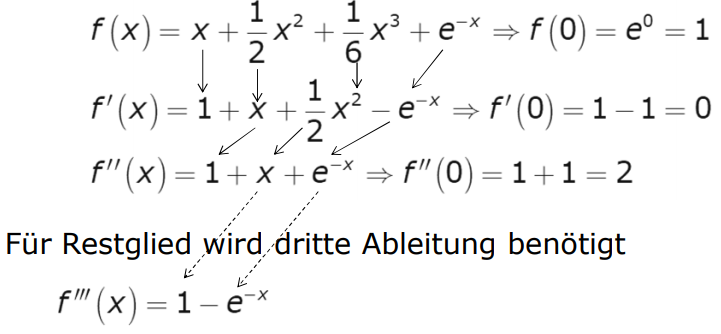
\includegraphics[width=0.7\textwidth]{Bilder/V1/30.png}\\
Für e gilt:\\
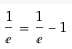
\includegraphics[width=0.1\textwidth]{Bilder/V1/31.png}\\
Jetzt alles in die Formel einsetzten:\\
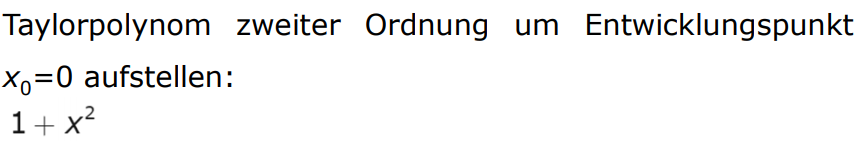
\includegraphics[width=0.8\textwidth]{Bilder/V1/32.png}\\
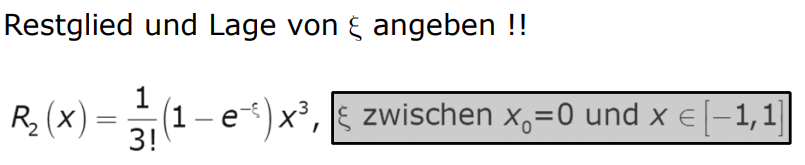
\includegraphics[width=0.8\textwidth]{Bilder/V1/33.png}\\
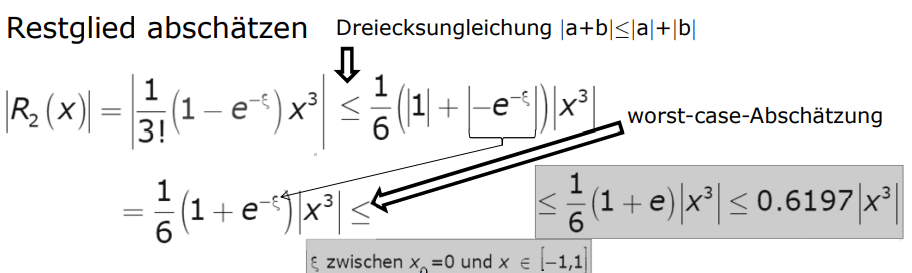
\includegraphics[width=0.8\textwidth]{Bilder/V1/34.png}\\
Worst Case, wäre XI gleich -1\\
\end{document} 

